\documentclass[]{article}

\usepackage{amsmath, amssymb} % Math formatting and symbols
\usepackage{graphicx} % Insert graphics
\usepackage{wrapfig} % Allow text to wrap around images
\usepackage[cm]{fullpage} % Smaller margins and header/footer
\usepackage{setspace}
\usepackage{gensymb} % degree symbol

\usepackage{float}

\usepackage{enumitem} % Allow for widest tag in enumerate

\renewcommand*\descriptionlabel[1]{\hspace\leftmargin$#1$}

\newenvironment{adescription}[1]
{\begin{list}{}%
		{\renewcommand\makelabel[1]{##1\hfill}%
			\settowidth\labelwidth{\makelabel{#1}}%
			\setlength\leftmargin{\labelwidth}
			\addtolength\leftmargin{\labelsep}}}
	{\end{list}}

\newcommand{\bd}{\textbf}
\newcommand{\dquad}{\quad{}\quad{}}

\title{\vspace{-5ex}Graph of Equations \vspace{-5ex}}
\author{}
\date{}

\begin{document}
	\setstretch{0.82}
	\maketitle{}
	
	\subsection*{}
	
	\subsubsection*{Set Notation}
	Roster Notation: $ A = \{ a, b, c \} $ or $ A = \{ a, b, c, ..., z \} $ \\
	Set Builder Notation: $ A = \{\,x \mid x \text{ is a lowercase character in the Latin alphabet }\,\}$
	
	\subsubsection*{Terminology and implications}
	Given sets...
	\begin{align*}
		A &= \{ a, b, c \} \\
		B &= \{ a, b, c, ..., z \} \\
		C &= \{ a, e, i, o, u \} \\
		D &= \{ a, i, u, e, o \} \\
		E &= \{ a, e, i \}
	\end{align*}
	We know
	\begin{align*}
		& a \in A              & &\text{a is an element of A} \\
		& e \notin A        & &\text{e is not an element of A} \\
		& A \notin A        & &\text{A set cannot be an element of a set} \\
		& \O = \{ \}           & & \\
		& U = \text{All elements of interest} & & \\
		& C = D               && \\
		& C \neq E          & & \\
		& E \subset C     & &\text{E is a proper subset of C} \\
		& E \subseteq C & &\text{E is a subset of C} \\
		& A \cup E = \{ a, b, c, e, i \} & &\text{A union E equals everything in A or E} \\
		& A \cap E = \{ a \} & &\text{A join E equals everything in A and E} \\
		& A^c = \{ d, e, f, ..., z \} & &\text{The compliment of A is all elements in the universal set and not in A}
	\end{align*}
	
	\subsubsection*{Laws and Properties}
	Commutative
	\begin{align*}
		A \cup B &= B \cup A \\
		A \cap B &= B \cap A
	\end{align*}
	Associative
	\begin{align*}
		A \cup (B \cup C) &= (A \cup B) \cup C \\
		A \cap (B \cap C) &= (A \cap B) \cap C
	\end{align*}
	Distributive
	\begin{align*}
		A \cup (B \cap C) &= (A \cup B) \cap (A \cup C) \\
		A \cap (B \cup C) &= (A \cap B) \cup (A \cap C)
	\end{align*}
	De Morgans Laws
	\begin{align*}
		(A \cup B)^c &= A^c \cap B^c \\
		(A \cap B)^c &= A^c \cup B^c
	\end{align*}
	
	\subsubsection*{Combinatorics}
	\begin{align*}
		n(S) &= \text{Number of unique items in set S} \\
		n(A \cup B) &= n(A) + n(B) - n(A \cap B) \\
		n(A \cup B \cup C) &=  n(A) + n(B) + n(C) \\
										 & - n(A \cap B) - n(A \cap C) \\
										 & - n(B \cap C) + n(A \cap B \cap C)
\end{align*}


	\subsection*{Graphing Trigonometric Functions}
	
	Assume... \\
	\indent $ y = d + a * f(bx - c) $ \\
	\indent Amplitude = $ \vert a \vert $ \\
	\indent Vertical Shift =$ d $ \\
	\indent Phase Shift = $ \frac{c}{b} $ \\
	\indent X-Scale (change between critical points) = $ \frac{\text{period}}{4} $ \\
	Period depends on what functions \\
	\indent sin, cos, csc, sec = $ \frac{2\pi}{b} $ \\
	\indent tan, cot = $ \frac{\pi}{b} $
	
	\subsubsection*{Examples...}
	
%	\begin{figure}[H]
%		\centering
%		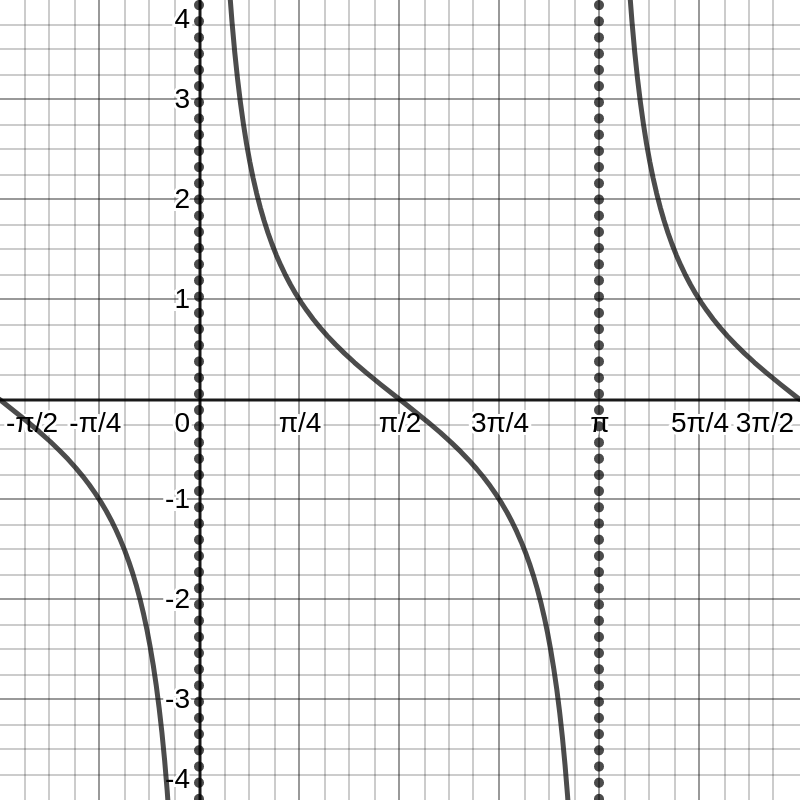
\includegraphics[width=0.20\textwidth]{cot.png}
%		\caption{$ y = \cot(x) $}
%	\end{figure}

\end{document}